\documentclass{beamer}
\mode<presentation>
\usepackage{amsmath}
\usepackage{amssymb}
%\usepackage{advdate}
\usepackage{graphicx}
\usepackage{adjustbox}
\usepackage{subcaption}
\usepackage{enumitem}
\usepackage{multicol}
\usepackage{mathtools}
\usepackage{listings}
\usepackage{url}
\def\UrlBreaks{\do\/\do-}
\usetheme{Boadilla}
\usecolortheme{lily}
\setbeamertemplate{footline}
{
  \leavevmode%
  \hbox{%
  \begin{beamercolorbox}[wd=\paperwidth,ht=2.25ex,dp=1ex,right]{author in head/foot}%
    \insertframenumber{} / \inserttotalframenumber\hspace*{2ex} 
  \end{beamercolorbox}}%
  \vskip0pt%
}
\setbeamertemplate{navigation symbols}{}

\providecommand{\nCr}[2]{\,^{#1}C_{#2}} % nCr
\providecommand{\nPr}[2]{\,^{#1}P_{#2}} % nPr
\providecommand{\mbf}{\mathbf}
\providecommand{\pr}[1]{\ensuremath{\Pr\left(#1\right)}}
\providecommand{\qfunc}[1]{\ensuremath{Q\left(#1\right)}}
\providecommand{\sbrak}[1]{\ensuremath{{}\left[#1\right]}}
\providecommand{\lsbrak}[1]{\ensuremath{{}\left[#1\right.}}
\providecommand{\rsbrak}[1]{\ensuremath{{}\left.#1\right]}}
\providecommand{\brak}[1]{\ensuremath{\left(#1\right)}}
\providecommand{\lbrak}[1]{\ensuremath{\left(#1\right.}}
\providecommand{\rbrak}[1]{\ensuremath{\left.#1\right)}}
\providecommand{\cbrak}[1]{\ensuremath{\left\{#1\right\}}}
\providecommand{\lcbrak}[1]{\ensuremath{\left\{#1\right.}}
\providecommand{\rcbrak}[1]{\ensuremath{\left.#1\right\}}}
\theoremstyle{remark}
\newtheorem{rem}{Remark}
\newcommand{\sgn}{\mathop{\mathrm{sgn}}}
\providecommand{\abs}[1]{$\left\vert#1\right\vert$}
\providecommand{\res}[1]{\Res\displaylimits_{#1}} 
\providecommand{\norm}[1]{\lVert#1\rVert}
\providecommand{\mtx}[1]{\mathbf{#1}}
\providecommand{\mean}[1]{E$\left[ #1 \right]$}
\providecommand{\fourier}{\overset{\mathcal{F}}{ \rightleftharpoons}}
%\providecommand{\hilbert}{\overset{\mathcal{H}}{ \rightleftharpoons}}
\providecommand{\system}[1]{\overset{\mathcal{#1}}{ \longleftrightarrow}}
%\providecommand{\system}{\overset{\mathcal{H}}{ \longleftrightarrow}}
	%\newcommand{\solution}[2]{\textbf{Solution:}{#1}}
%\newcommand{\solution}{\noindent \textbf{Solution: }}
\providecommand{\dec}[2]{\ensuremath{\overset{#1}{\underset{#2}{\gtrless}}}}
\newcommand{\myvec}[1]{\ensuremath{\begin{pmatrix}#1\end{pmatrix}}}
\let\vec\mathbf

\lstset{
%language=C,
frame=single, 
breaklines=true,
columns=fullflexible
}

\numberwithin{equation}{section}

\title{3.3.8}
\author{AI25BTECH11024 - Pratyush Panda}
\begin{document}
\maketitle

\begin{frame}
\textbf{Question: } \\
Construct a triangle $\Delta ABC$ with side $BC = 7 cm$, $\angle B=45^\circ$, $\angle A=105^\circ$.
\end{frame}

\begin{frame}
\textbf{Solution: } \\
Let the position vector of $\Vec{B}$ be $\myvec{0 \\ 0}$ and the position vector of $\Vec{C}$ be $\myvec{7 \\ 0}$ as $BC=7cm$ is given.\\
Let a, b and c be the length of sides opposite to the vertex A, B and C respectively.

Now, we know that sum of all interior angles of a triangle is $180^\circ$, thus;
\begin{align}
\angle A + \angle B + \angle C = 180^\circ
\end{align}
\begin{align}
or \, 105^\circ + 45^\circ + \angle C = 180^\circ
\end{align}
\begin{align}
Thus, \, \angle C = 30^\circ
\end{align}

We can form two equations to get the other two sides such as;
\begin{align}
b\cos C + c\cos B = 8
\end{align}
\begin{align}
b\sin C - c\sin B = 0
\end{align}
\end{frame}

\begin{frame}
On writing this system of equation as a matrix equation, we get;
\begin{align}
\myvec{\cos C & \cos B \\
       \sin C & -\sin B}
\Vec{X} = 
\myvec{7 \\ 0} \, \textit{where } \Vec{X}=\myvec{b \\ c}
\end{align}

After putting the values of all the trigonometric values, we get;
\begin{align}
\myvec{\frac{\sqrt{3}}{2} & \frac{1}{\sqrt{2}} \\
       \frac{1}{2} & -\frac{1}{\sqrt{2}}}
\Vec{X} = 
\myvec{7 \\ 0}
\end{align}

Now we can do row operations to get the Echelon form of this matrix.
\begin{align}
\myvec{\sqrt{3}/2 & 1/\sqrt{2} \\
    0 & (-\frac{1}{\sqrt{2}} - \frac{1}{\sqrt{6}}}
\Vec{X} = 
\myvec{7 \\ \frac{7}{\sqrt{3}}}
\end{align}

On solving this equation we get;
\begin{align}
\Vec{X} = \myvec{7\brak{\frac{1-\sqrt{3}}{\sqrt{3}}} \\ \frac{7\sqrt{2}}{\sqrt{3}-1}}
\end{align}
\end{frame}

\begin{frame}
From here we get, $c=\frac{7\sqrt{2}}{\sqrt{3}-1}$ \\

Now, the coordinates of $\Vec{A}$ can be written as;
\begin{align}
\Vec{A}=\myvec{c\cos B \\ c\sin B}
\end{align}
\begin{align}
or, \, \Vec{A}=\myvec{\frac{c}{\sqrt{2}} \\ \frac{c}{\sqrt{2}}}=\myvec{\frac{7}{\sqrt{3}-1} \\ \frac{7}{\sqrt{3}-1}}
\end{align}
Now, we can plot the triangle using the three points.
\end{frame}

\begin{frame}
\begin{figure}[H]
\centering
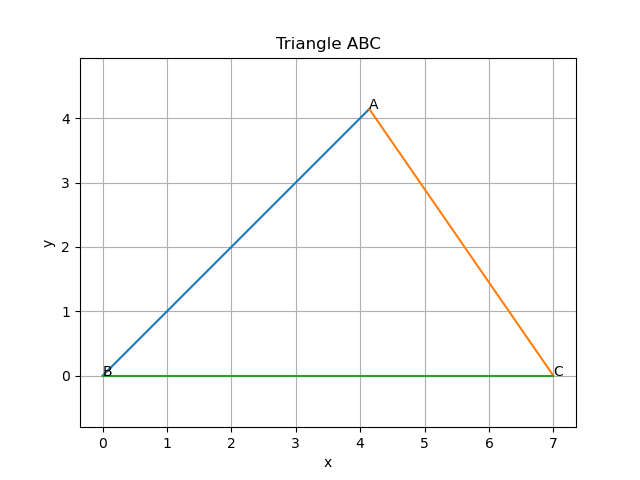
\includegraphics[width=0.8\columnwidth]{figs/img.png}
\caption*{}
\end{figure}
\end{frame}

\end{document}